\section{提案}
本研究では,Android を標的にしたマルウェアの動的解析を行う.マルウェアにログコードを挿入させ,そのログを動的に得ることで解析を行う.エミュレータでは再現できないために解析できないことも,本提案を適用することで,実機でマルウェアを動かすため解析できるというメリットがある.\ref{overview} では,本提案の全体の流れを説明する.\ref{analysismethod} では,本提案の解析手順を,\ref{placeinsert} では,ログコードをどこに挿入するかについて説明する.

\subsection{概要}
\label{overview}
本研究で対象とする Android アプリのマルウェアを解析するためにはメソッドの情報が必要である.解析を行っていくためには,マルウェアがどのようなコードが実行したかということを知る必要がある.Android アプリのマルウェアは Java で実装されているため,解析の手がかりとなるのはメソッドのログである.このログにはマルウェアがどんなメソッドを実行したかという情報とそれぞれのメソッドについての情報が含まれている.メソッドの情報とは具体的にいうと,メソッド名,そのクラス名,引数の型名と値である.本提案では,このログを用いてマルウェアの解析を行う.

本提案では,先に述べたログを得るためにマルウェアのメソッドにログを出力させるコードを挿入する.Android API では,デバッグ用等のために,ターミナルにログを出力する API を提供している.その API とは android.util.Log である.以下に示す例のようなコードをメソッドの中に挿入する.Log.d の ".d" は "DEBUG" を表しており,Android のログの重要度を示している.ログコードを挿入してマルウェアを実行させると,マルウェアがそのメソッドを実行したときにそのログコードは必ず実行される.よってメソッドについてのログを出力させることができる. \ref{analysismethod} では,どのようにコードを挿入するかの手順について説明する.

\begin{itembox}[l]{android.util.Log の例}
	Log.d("Tag", "Log Message");
\end{itembox}

本提案では,まずマルウェアの APK ファイルを入手することから始まる.次に,APK ファイルから Java クラスファイルを取り出し,ログをターミナルに出力させるためのコードを挿入する.このログには,実行したメソッド名,そのメソッドの引数の型名とその値を出力させるようにする.コードを挿入するとは,マルウェアから取り出した Java クラスファイルを書き換えるということである.マルウェアにコードを挿入した後,書き換えた Java クラスファイルを DEX コードに変換し,classes.dex を作成する.classes.dex を作ったら,元の APK ファイルの中にあるオリジナルの classes.dex とコードが挿入されている新しい classes.dex を入れ替える.ログコードを挿入したマルウェアを Android 端末にインストールした後,DDMS (Dalvik Debug Monitor Server) というツールを用いることで,Android OS が出す多数のログの中からマルウェアが出したログを抜き取る.図 \ref{examplelog} は Android OS が出力するログの例である.先に示した android.util.Log の例で示したように,それぞれのログにはタグがある.例を出すと,図 \ref{examplelog} の 3 つめのログのタグは "UploadsManager" であることがわかる.さらに,一番左の項目は "D"  となっていることから,このログの重要度は "DEBUG" レベルであることがわかる.Android のログのタグは自分自身で決めることができるので,このタグを使って,本提案によるマルウェアのログのみを得ることができる.マルウェアのログを得ることで,マルウェアが実行したメソッドとその情報がわかるので,そこからマルウェアの挙動を解析できる.

\begin{figure}[t]
\begin{center}
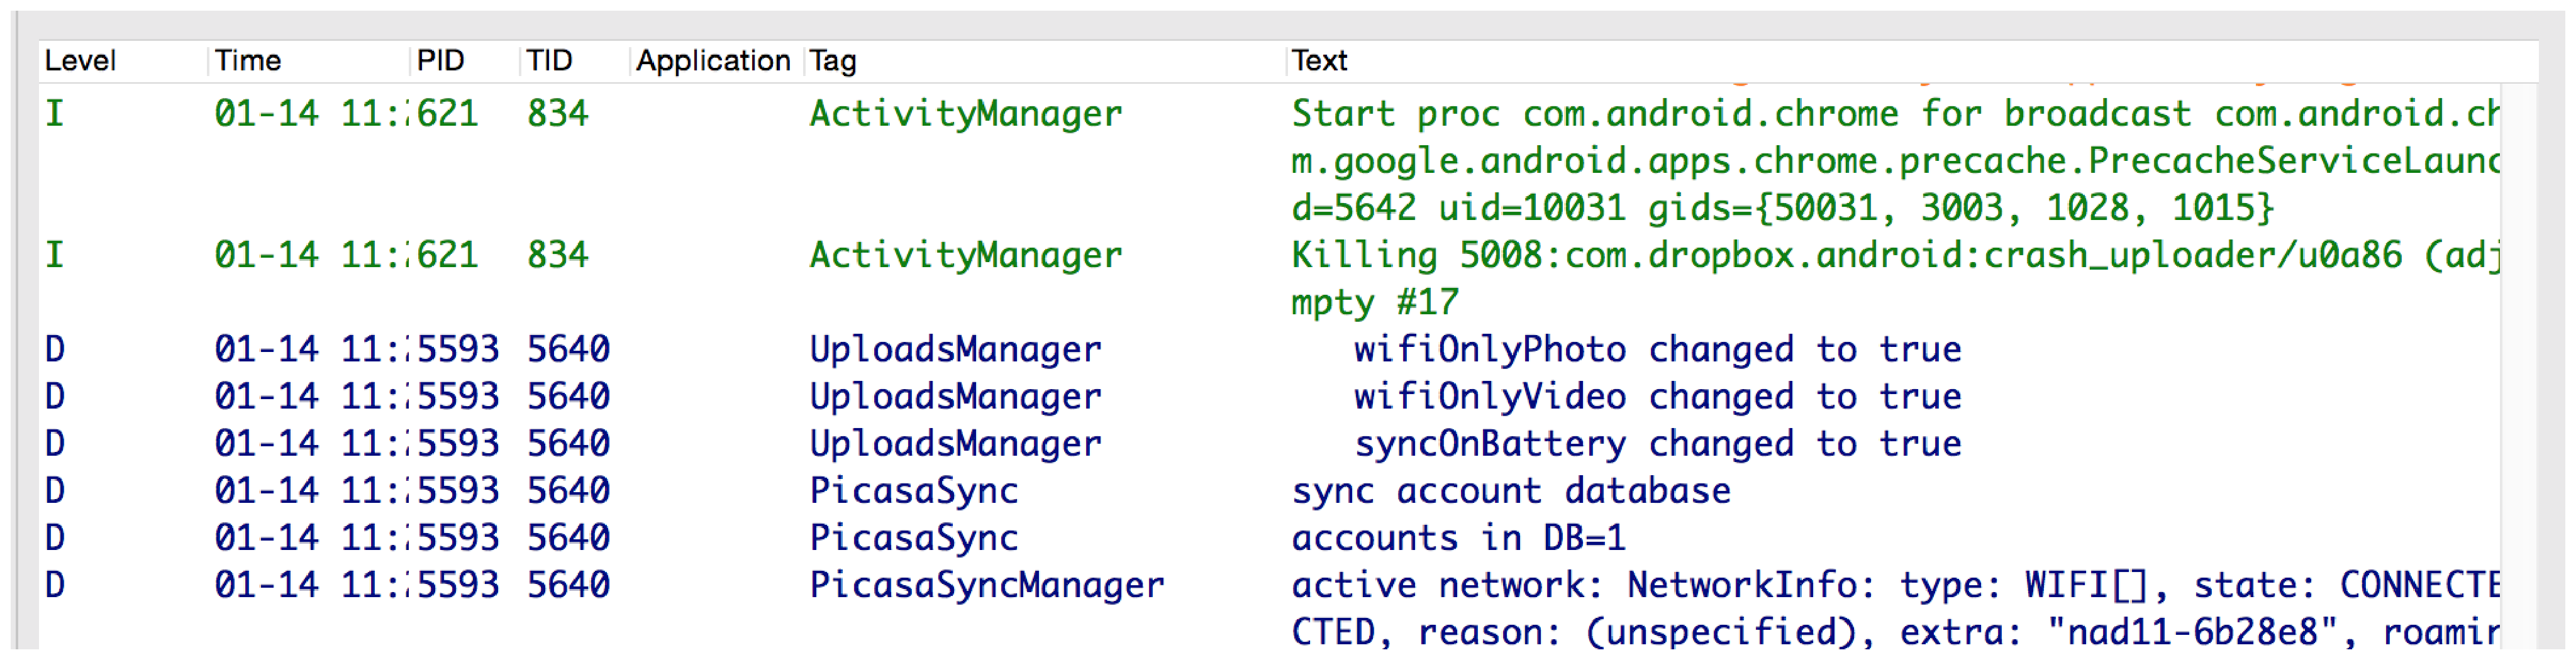
\includegraphics[scale=0.2]{androidlogexample.eps}
\end{center}
\caption{Android が出力するログの例}
\label{examplelog}
\end{figure}

\subsection{解析手順}
\label{analysismethod}
最初に,大まかな手順の流れを説明する.Step 1 で,APK ファイルから Java クラスファイルを取り出す. Step 2 では,その Java クラスファイルにログコードを挿入する.Step 3, 4  でそのログコードを挿入した APK ファイルを作成し,実機にインストールする.その後,マルウェアを起動して,ログを得る (Step 5, 6). 以下にそれぞれの Step の詳細な説明をする.

[Step1] まず最初の手順として,APK ファイルから Java クラスファイルを取り出す.\ref{sec:andrapp} で述べたように,APK ファイルを解凍することで,classes.dex を得ることができる.classes.dex からJava クラスファイルを取り出すために,dex2jar \cite{d2jar} が提供する sh プログラム (d2j-dex2jar.sh)を用いる.これにより, DEX コードファイルを JAR ファイルに変換することができる.よって,APK ファイルを解凍して出てきた classes.dex から dex2jar を用いて 1 つの JAR ファイルを得ることができる.この JAR ファイルを解凍することで Android アプリの Java クラスファイルを得る.

[Step 2] マルウェアの Java クラスファイルを得た後は,これにログを出力するコードを挿入する.つまりマルウェアの Java クラスファイルを書き換える.本研究では,Java クラスファイルを書き換えるために Javassist \cite{javassist} という Java ライブラリを用いる.Javassist は Java バイトコードの知識があまりなくても バイトコード変換のための API を提供する Java ライブラリである.Java で実装したプログラムでマルウェアの Java クラスファイルを書き換える.実装したプログラムについては,\ref{sec:instrument} 章で詳しく説明する.

[Step 3] Java クラスファイル を書き換えた後は,classes.dex を作成する.classes.dex を作成するためには,複数のクラスファイルを JAR ファイルにまとめる必要がある.dex2jar で得た JAR ファイルを解凍した際に,ディレクトリがいくつも出てくる場合がある.その場合は,ディレクトリ毎に JAR ファイルにまとめ,ディレクトリに属していないクラスファイルだけで,ひとつの JAR ファイルにまとめる. そして,以下に示すコマンドで JAR ファイルから classes.dex を作成する.dx とは,Android SDK が提供する dx コマンドのことである.このコマンドにより,JAR ファイルから DEX コードの変換を行う.

\begin{itembox}[l]{JAR ファイルから classes.dex を作る dx コマンド}
	dx --dex --output="classes.dex" "direcA.jar" "direcB.jar" 
\end{itembox}

[Step 4] 次に,新しく作成した classes.dex を APK ファイル内にあるオリジナルの classes.dex と入れ替え.端末にインストールできるように APK ファイルにサインを行う.先に述べたように,APK ファイルは ZIP 形式であるから, zip コマンドに -u オプションをつけることで,新しいファイルを古いものと入れ替えることができる.APK ファイルにサインするためには,dex2jar の中の d2j-apk-sign.sh を用いる.例えば,sampleApp.apk に対してこのプログラムを実行すると,sampleApp\_signed.apk のように別の新しい APK ファイルが生成される.そして,adb shell を使って,この APK ファイルを実機にインストールする.

[Step 5] マルウェアのインストール後,手動でそのマルウェアを起動し,DDMS に出力されるマルウェアのログをテキストファイルに保存する.Android OS が出力しているログは,ターミナルでも見ることができるが,細かい内部システムの状態などの情報が大量に出てくる.そのため,マルウェアが出しているログをそこから見つけることは困難である.DDMS では,指定したタグのみを出力することができる.マルウェアに挿入するコードには,タグを自分で指定しているため,DDMS にはマルウェアの実行ログのみを表示することができる.そして,表示されているログをテキストファイルとして保存する.

[Step 6] さらに,ログをより解析しやすくするために,このマルウェアのログのテキストファイルをクラス毎に分割する.なぜなら,そのままの状態では,複数のクラスのメソッドのログが混在していて,何が行われているか理解しにくいためだ.ログをパースするスクリプトを実装し,それを得られたテキストファイルに適用し,クラス毎に分割した.このスクリプトについては, \ref{sec:instrument} 章で詳しく説明する.

\subsection{ログコードの挿入箇所}
\label{placeinsert}
マルウェアの挙動を解析するためには,ログコードを適切な箇所へ挿入する必要がある.そこで本節では,マルウェアの Java クラスファイルへログコードを挿入する際に,どのような箇所へ挿入するか,どのような情報をログコードで出力させるかについて説明する.\ref{methodtop} では,メソッドの先頭へのコード挿入について,\ref{methodcalls} では,メソッド呼び出しの前後でのコード挿入について,なぜそこへ挿入するかという理由も含めて説明する.

\subsubsection{メソッドの先頭へのコードの挿入}
 \label{methodtop}
メソッドの先頭へログコードを挿入するのは,メソッドが実行された時に,そのログコードを確実に実行しそのログを出力させるためである.Javassist が提供する API では,メソッドの先頭か,最後にコードを挿入できる.メソッドの最後にコードを挿入してしまうと,メソッドが実行されたときに,そのコードが確実に実行されるかどうかは分からない.理由は主に 2 つ考えられる.1 つは,メソッドの途中で return 文が書かれている場合である.if 文の中で return 文が書かれていて,ある条件ではその if 文が実行されて,メソッドの最後まで到達せずに呼び出し元へ返ってしまい,メソッドの最後にあるログコードは実行されなくなってしまう.また,マルウェア作成者が解析者の混乱を誘うために,意図的にメソッドの途中で return 文を置いている可能性もある.もう一つの理由は,そのメソッドが途中で他のメソッドを呼び出してそのメソッドの最後まで到達しない場合だ.例えば メソッド A,B の最後にログコードを挿入し,メソッド A の中でメソッド B を呼びだすというケースを考える.そして,メソッド B の中でそのアプリが終了する関数が最後に呼ばれたとする.そうすると,メソッド A だけでなく,メソッド B のログコードも実行されなくなってしまう.なぜなら,メソッド B のログコードはアプリを終了させる関数の後に挿入されることから,このログコードは実行されないからだ.もし実行フローが最後まで到達して,ログコードが実行されたとしても,解析する際には時系列とは逆の順番でログが出力されるので紛らわしくなってしまうというデメリットもある.メソッドの先頭へログコードを挿入するイメージ図 \ref{insertbefore} を以下に示す.図 \ref{insertbefore} が示すように各メソッドのメソッド先頭,つまりそのメソッドが実行された場合,この挿入されたコードが一番最初に実行されるということになる.よって,メソッドの先頭にログコードを挿入すると,メソッド内の条件等にかかわらず,必ずそのログコードが実行されることになる.

\begin{figure}[t]
\begin{center}
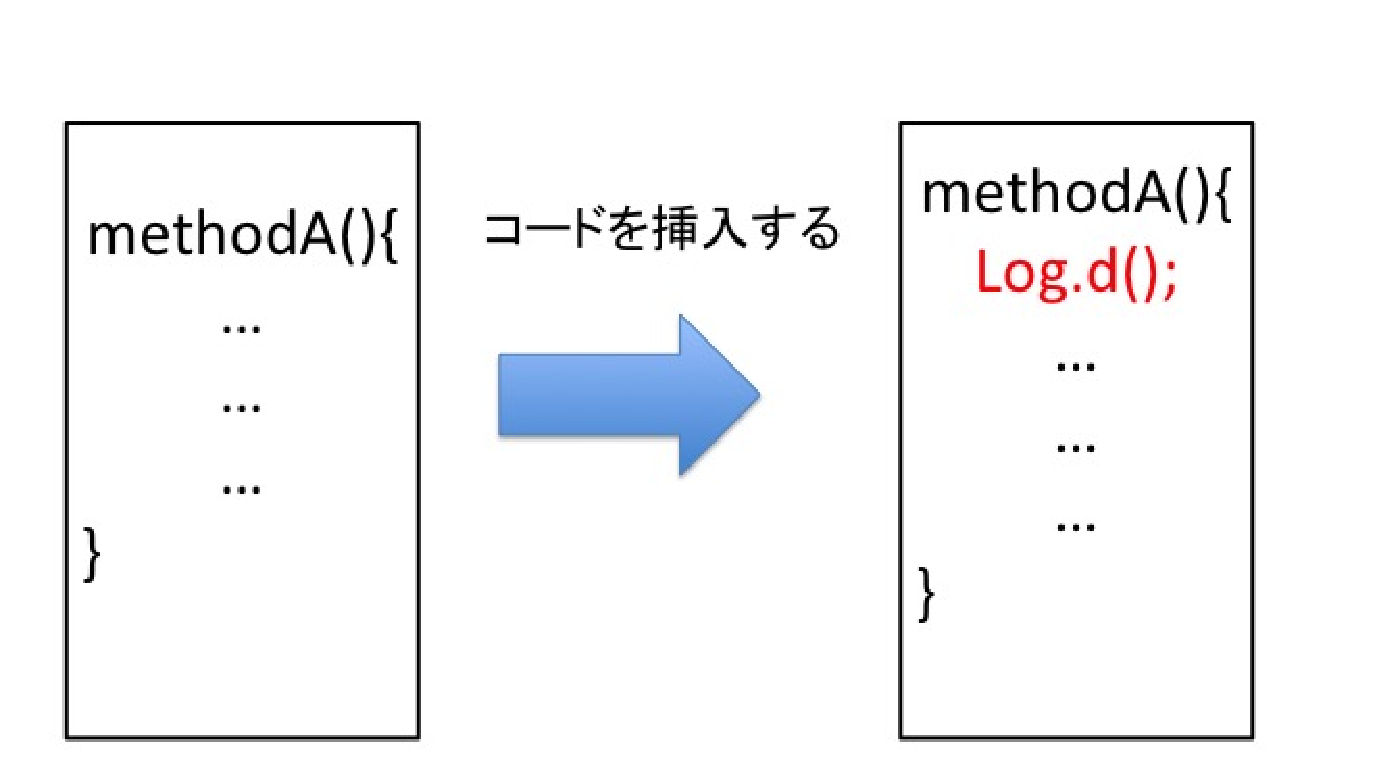
\includegraphics[scale=0.3]{image2.eps}
\end{center}
\caption{メソッドの先頭へコードを挿入するイメージ図}
\label{insertbefore}
\end{figure}

メソッドの先頭に挿入するログコードではクラス名,メソッド名,そのメソッドの引数の情報を出力させる.メソッドの引数の情報とは,引数の型名とその引数の値である.なぜ引数の型名だけでなく,中身を出力させるかというと,引数の中身がわかるとマルウェアの挙動がより見えやすくなるからである.例えば,メソッド名が "getCode",メソッドの引数の 1 つの型が String 型とわかっていたとする.しかし,これだけでは,String の中身がどんなものなのかよくわからない.なぜなら,String 型の変数はいろんな使われ方が考えられるからだ.型名だけで類推することはできても特定するのはとても困難である.この引数はサーバからのコマンドや,盗んだ端末についての情報の文字列かもしれない.そこで,引数の具体的な値が,URL のような文字列であることがわかると,この引数はコードを取ってくるアドレスということである確率がとても高いといえる.同様なことが int 型の場合も考えられる.もし int 型のメソッドの引数が携帯電話の番号(11 ケタで,090 や 080 で始まっている数字列)だった場合,そのマルウェアは感染した端末の電話番号を盗んでいたり,SMS をバックグラウンドで送信している可能性が出てくる.たとえメソッド名がマルウェア作成者により意図的に変えられていたとしても電話番号を引数にとっているということは端末の情報への不正なアクセスを明らかに示している.このようにメソッドの引数の値はマルウェアを解析するにあたって重要な要素であり,この情報によって解析がより行いやすくなる.

しかしこの手法を適用できないメソッドが 2 種類ある.
1 つは java.lang に属するクラスである.たとえば,String クラスのメソッドである,toString() の先頭にはログコードを挿入することはできない.Javassist の API では,JVM にすでにロードされているクラスのクラスファイルは書き換えることができないという制限がある.そのため,Java のプログラムが実行時(この場合,クラスファイルを書き換えようとしている時)には,JVM には java.lang.String クラスがロードされているため,Javassist は String  クラスのクラスファイルを書き換えることはできない.この手法を適用できないもう一つのメソッドの種類は Android API である.Android API は Android システムの内部に組み込まれているため,Java クラスファイルとしては存在していない.Javassist は Android の内部に組み込まれているものを操作できないため,Javassist では,これらのメソッドの先頭にコードを挿入することはできない.マルウェアをより詳細に解析していくためには,メソッドの先頭へログコードの挿入は不十分である.この問題を解決するために, \ref{methodcalls} の手法を利用する.

\subsubsection{メソッド呼び出しの前後でのコードの挿入}
\label{methodcalls}
マルウェアをより深く解析していくために,メソッド呼び出しの前後にログコードを挿入する.図 \ref{insertbetw} はメソッドの前後にコードを挿入するイメージ図である.この図が示すように,呼び出されるそれぞれのメソッドの前後にログコードを挿入する.
この図では,methodA の中で,methodB, methodC が呼び出されている.methodA が実行されたとすると,methodB, methodC の実行の前後にそれぞれのメソッドについてのログが出力されることになる.つまり,あるメソッド内でどのようなメソッドが呼び出されているかがわかるようになる.

メソッドの前後にログコードを挿入する場合は \ref{methodtop} の手法とは異なる Javassist の API を用いるため,\ref{methodtop} の手法では適用できない2 種類のメソッドについてのログを出力することができる.つまり,あるメソッドの中で java.lang のクラスのメソッドや,Android API が実行されたということがわかるようになる.図 \ref{insertbetw} の methodB または methodC が java.lang.String  クラスの toString() であってもこの手法を適用することができる.メソッド呼び出しの前後にログコードを挿入することで,より多くのメソッドについてのログが出せるようになり,あるメソッド内でどんなメソッドが実行されたかが明らかになる.

\begin{figure}[t]
\begin{center}
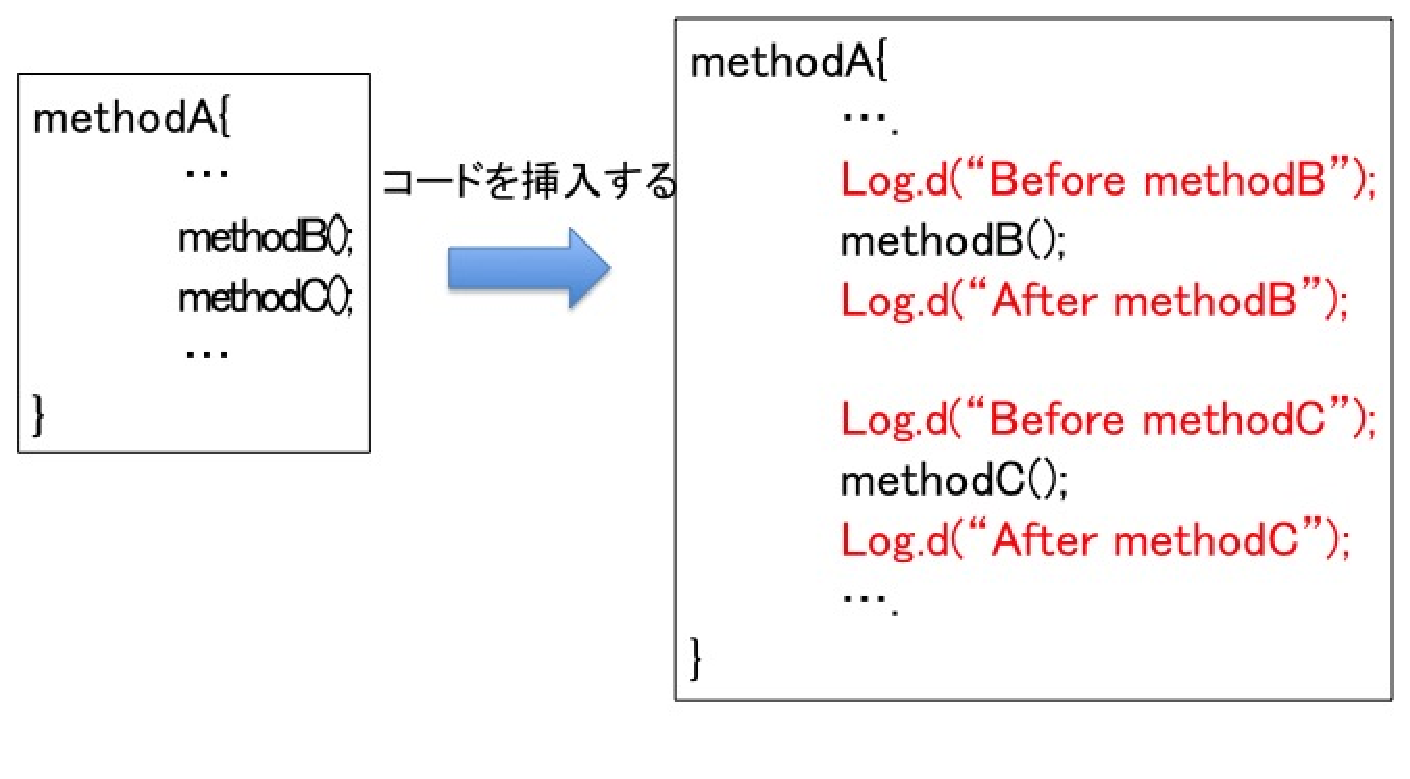
\includegraphics[scale=0.35]{image4.eps}
\end{center}
\caption{メソッドの前後にコードを挿入するイメージ図}
\label{insertbetw}
\end{figure}

\begin{figure}[t]
\begin{center}
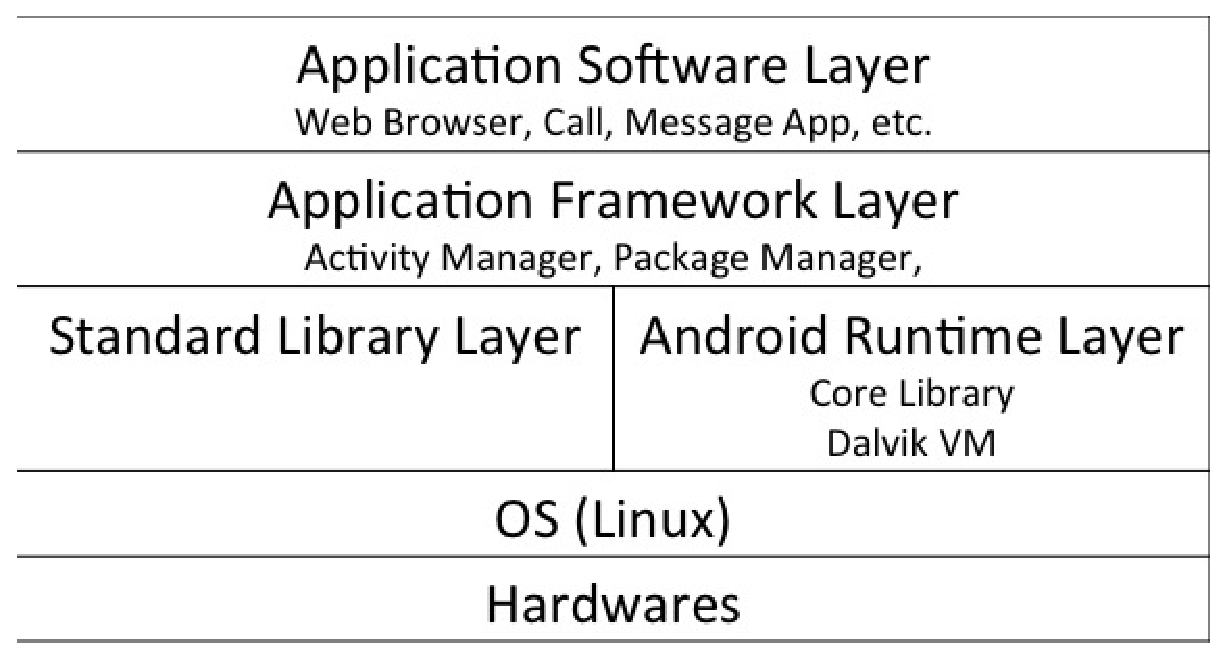
\includegraphics[scale=0.5]{structure2.eps}
\end{center}
\caption{Android の内部構成}
\label{structure}
\end{figure}

呼び出されるメソッド呼び出しについてのログには,それ自身はもちろんのこと,呼び出し元のメソッドの情報も出力させる.呼び出し元のメソッドの情報はマルウェアの解析に必要である.なぜなら,マルウェアの解析を行うにあたり,どのメソッドがどこから呼び出されたかを知る必要があるからだ.どこから呼び出されたかがわからないと,ただそのメソッドが実行されたということしかログからは知り得ない.例えば,クラス A のメソッド mA とクラス C のメソッド mC の 2 つのメソッドからクラス B の mB が実行される場合を考える.もし,呼び出し元の情報がないと,クラス B の mB の実行ログを得ても,クラス A のメソッド mA からなのか,クラス C のメソッド mC から呼び出されているかがわからない.

また,\ref{methodtop} の方法では,プログラムの実装の都合や Javassist のAPI の都合上,呼び出し元をログとして出力させることはできない.\ref{sec:instrument} 章で説明するように,メソッドの先頭に挿入するプログラムのアルゴリズムでは,呼び出し元の情報を得る機能を追加することはできないためだ.この場合については,メソッドへのコードを挿入せずに,メソッド呼び出しの置き換えを行っている.この置換えによって,メソッドのオブジェクト(javassist.expr.MethodCall クラスのオブジェクト ) を得られる.MethodCall クラスのオブジェクトの情報から呼び出しているメソッド名,そのメソッドのクラス名を取得することができる.

